\documentclass[11pt]{article}
\usepackage[margin=1in]{geometry}
\usepackage{amsmath,amssymb,booktabs,microtype,graphicx,xcolor}
\usepackage[round]{natbib}
\usepackage[colorlinks=true,linkcolor=blue!50!black,urlcolor=blue!50!black,citecolor=blue!50!black]{hyperref}
\setlength{\parskip}{0.35em}\setlength{\parindent}{0em}
\title{\textbf{How Much Tail Prediction Could We Have Detected?\\
A Power Accounting for a 1,450-Test Search}}
\author{Charlie Yan\thanks{Draft v0.3 (journal-length), August 2026. All statistics
\textsc{screen}-basis: information coefficients and event classification. No performance
claims appear in this paper. The detectability table and Exhibit~1 are produced by a
checked-in script (\texttt{p3\_power\_table.py}), not by in-text arithmetic.
Code, pre-registration documents and a data-availability statement: \url{https://github.com/charlieyanhx/tail-power-accounting}.}}
\date{August 2026}
\begin{document}\maketitle

\begin{abstract}
We searched eight feature families---intraday microstructure, skew structure, quote geometry,
event anatomy, funding spreads, cross-asset carry, GARCH/EVT states, and sector-rotation
dispersion---for predictors of the left tail of a short-volatility options book: roughly 1{,}450
tests against a fixed pre-registered target panel, with adversarial re-verification of every
near-miss. Zero survived the family-wise bar. This paper argues that such a null is nearly
uninterpretable unless the searcher also reports what the search \emph{could} have found, and
supplies that accounting. The honest unit of the tail sample is not the 1{,}237 rows of the
target panel (1{,}168 of which carry both a complete ten-day forward window and the trailing
volatility normalizer) but approximately fifteen distinct loss episodes, and the accounting
therefore runs on two levels. Deflating daily rows for overlapping horizons, the search had
80\% power at the Bonferroni-adjusted threshold only against true tail information coefficients
of $|IC| \ge 0.46$ at the ten-day horizon and $\ge 0.34$ at five days; clustering at the
episode level---the unit the census below says carries the information---the certifiable floor
rises to $|IC| \approx 0.77$--$0.91$, and event-level classifiers were certifiable only above
an area under the ROC curve of 0.86. The best graded candidates sat at 0.21--0.23: half the
day-level threshold, a quarter of the episode-level one, and approximately the expected maximum
of 1{,}450 null draws at these effective sample sizes. The correct conclusion is therefore a
bound: either any true separator in the tested families is weaker than these thresholds---which
sit well above the sustained daily-horizon effect sizes the positioning and flow literature
reports---or it was not among the tested features. Two structural findings sharpen the bound and survive it. First, a census
of the fifteen episodes shows only two began from a calm state; the other thirteen were
preceded by elevated generic risk states that carry conditional \emph{means} three to thirteen
times baseline in every year of the sample---so the states that forecast the tail also forecast
the premium, and no walk-forward de-sizing overlay we tested shows a demonstrable net gain
(every improvement interval contains zero). Second, protection was 4--16\%
more expensive precisely when candidate separators fired: the market charges for the same
information at the moment it becomes available. We propose that tail-signal searches publish
this power accounting as standard practice, and offer a registered ratio of tail-IC to mean-IC
against an explicit forward-mean confound target as a pre-registration gate that removes the
premium-confound false positives which otherwise dominate such searches (the form transfers;
our threshold of 2 is a judgment calibrated on this search).
\end{abstract}

\section{Why a null needs a power statement}
Negative results in quantitative finance are published rarely and read sceptically, and the
scepticism is usually well founded: ``we looked and found nothing'' is consistent with there
being nothing to find, with looking in the wrong place, and with looking with an instrument too
blunt to see what is there. Only the first is a scientific claim. Distinguishing them requires
the searcher to state, before or alongside the result, the smallest effect the search could
have certified.

For tail prediction this matters more than usual, because the effective sample is far smaller
than the nominal one in two compounding ways. Overlapping multi-day targets deflate independent
observations by roughly the horizon; and the events of interest---the days a
short-volatility book actually loses badly---are rare by construction. A study reporting
a four-figure observation count and a Bonferroni correction over a large test ledger sounds rigorous
and may in fact be nearly powerless. This paper supplies that accounting for one such search
and argues it should be routine.

\section{The search}
The target panel fixes, per trading day: forward five- and ten-day downside semivolatility, the
forward minimum, the worst single-day loss in units of trailing volatility, a tail-event
indicator, and---critically---the forward \emph{mean} over the same window, as an explicit
confound target. The panel spans 2020-12-11 to 2025-09-08 (1{,}237 trading days) and is the
mark-to-market daily series of a short-volatility SPY options book; the panel was frozen
roughly eight months before the end of the underlying 2020-09 to 2026-05 data sample, and
extending it would add rows but few episodes. Of the 1{,}237 rows, 1{,}227 carry a complete
ten-day forward window (the last ten rows do not) and 1{,}168 also carry the trailing 250-day
volatility normalizer that the $\sigma$-scaled targets require (the first 59 rows precede its
warm-up); the power accounting below uses the 1{,}168. Information coefficients are rank
(Spearman) correlations, residualized on declared controls. Features were
drawn from eight families and tested as information coefficients against the tail targets at
horizons of five and ten days, with family-wise error controlled by Bonferroni across a
declared ledger of roughly 1{,}450 tests (two-sided), and with every near-miss re-derived
independently by a second implementation before being graded.

The economics matter for interpreting the bar. The book being protected is short volatility, so
the payoff to a true separator is de-sizing before losses. The cost of a false one is forfeited
premium---and in this sample the richest sub-period is the \emph{non-acute} portion of stress
episodes, which is precisely when a naive risk-state signal would have the book standing down.
A tail signal must therefore not merely predict losses; it must predict them in a way that is
separable from the premium it would cause the book to forgo. Section~\ref{sec:gate} turns that
requirement into a testable gate.

\section{The power accounting}\label{sec:power}
\textbf{Overlap deflates the sample---and episode clustering deflates it further.} The
accounting runs on two levels, and we present both because they answer different objections.
At the day level, overlapping $h$-day targets leave roughly $n/h$ independent observations: at
$n = 1{,}168$ usable daily rows, $n_{\mathrm{eff}} \approx 116$ at $h = 10$ and $\approx 233$
at $h = 5$. But the abstract's own argument---that the honest unit is the loss episode---implies
the day-level figures are optimistic for the quantity that matters: if tail-relevant variation
is concentrated in roughly fifteen episode-level draws, the binding effective sample is nearer
15--30. We therefore quote the day-level floors as lower bounds and the episode-level floors as
the honest headline. The $n/h$ deflation is itself only adequate for target-side overlap: with
persistent regressors---risk states, volatility levels, exactly the candidates here---the
long-horizon regression literature shows effective information can be worse still
\citep{valk, brw}. Every approximation in Table~\ref{tab:power} therefore errs toward
understating the thresholds, which strengthens the bound.

\textbf{The detection threshold.} Under the Fisher transform for rank correlations,
$\mathrm{se} \approx 1.06/\sqrt{n_{\mathrm{eff}} - 3}$ (the 1.06 is the Spearman variance
factor). With a two-sided Bonferroni critical value $z_\alpha = 4.14$ at
$\alpha = 0.05/1{,}450$ and $z_{0.8} = 0.84$ for 80\% power,
\begin{equation}
|IC|_{\min} \;\approx\; \tanh\!\Big(\frac{1.06\,(z_\alpha + z_{0.8})}{\sqrt{n_{\mathrm{eff}} - 3}}\Big).
\label{eq:power}
\end{equation}
\begin{table}[h]\centering\small
\begin{tabular}{llccc}\toprule
Accounting & Unit & $n_{\mathrm{eff}}$ & $|IC|_{\min}$, Bonferroni $+$ 80\% power & $|IC|_{\min}$, nominal 5\% \\
\midrule
Day-level & 10-day horizon & $\approx 116$ & $\approx 0.46$ & $\approx 0.27$ \\
Day-level & 5-day horizon & $\approx 233$ & $\approx 0.34$ & $\approx 0.19$ \\
Episode-level & 15 episodes & 15 & $\approx 0.91$ & $\approx 0.70$ \\
Episode-level & 30 episodes & 30 & $\approx 0.77$ & $\approx 0.52$ \\
\bottomrule\end{tabular}
\caption{Smallest detectable tail information coefficient, from Equation~\eqref{eq:power}.
The day-level rows deflate the 1{,}168 usable daily rows by the target horizon; the
episode-level rows take the loss episode as the independent unit, which is what the census of
Section~4 argues. The two bracket the search's true blindness; the episode rows are the
binding ones if tail information is episode-concentrated.}
\label{tab:power}\end{table}
\begin{figure}[h]\centering
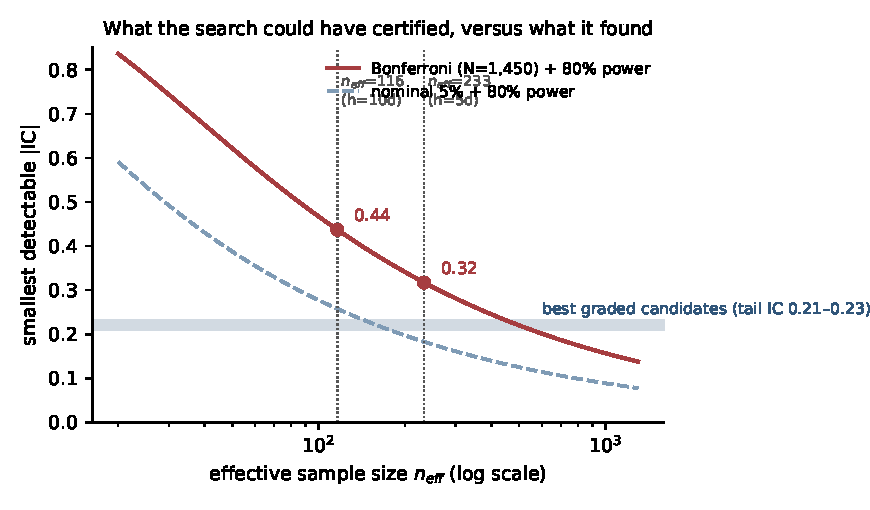
\includegraphics[width=0.72\textwidth]{fig_p3_power.pdf}
\caption{Exhibit 1. The day-level detectability frontier against effective sample size, with
the search's two operating points and the band occupied by its best graded candidates. The
candidates sit at roughly half the day-level certifiable threshold---and at approximately the
expected maximum of the search's own null distribution, which is why they are graded
uncertifiable. The episode-level operating points of Table~\ref{tab:power} lie further left,
off this frontier's favorable end.}
\label{fig:power}\end{figure}

\textbf{Event classification is harsher still.} Treating the problem as classification rather
than correlation, with $n_1 \approx 15$ loss episodes against $n_2 \approx 1{,}150$ ordinary
days, the Hanley--McNeil standard error \citep{hm} under the null ($\mathrm{AUC} = 0.5$) is
0.075, so the Bonferroni critical value is 0.811; requiring 80\% power against that critical
value (the alternative's standard error is smaller, e.g.\ 0.073 near $\mathrm{AUC} = 0.75$)
puts the certification floor at $\mathrm{AUC} \ge 0.862$.\footnote{An earlier draft quoted
0.828, computed with the alternative-hypothesis standard error in the rejection threshold;
the correction raises the floor and is in the checked-in script.} For calibration:
that is a classifier that ranks a randomly chosen loss episode above a randomly chosen ordinary
day roughly six times in seven, on daily data, out of sample. Rather than assert that no such
feature exists---a claim we cannot support without a systematic review---we note the implied
effect size: under a binormal model at this class imbalance, an AUC of 0.862 corresponds to a
point-biserial correlation of roughly 0.17, about twice the strongest positioning feature we
have ever documented on this data ($|IC| \approx 0.08$). A reader who knows of
a feature at this level has, by the same accounting, identified something the search would
indeed have found. (Hanley--McNeil also assumes independent observations; volatility
clustering among the ordinary days inflates the true standard error and hence the floor
further---one more approximation whose direction strengthens the bound.)

\textbf{What the null therefore means.} The best graded candidates in the search---a
quote-geometry feature and a sector-rotation dispersion measure, each with tail IC in the
0.21--0.23 range and a coherent mechanism---sit at about half the day-level threshold and a
quarter of the episode-level one. Two honesty notes attach. First, 0.21--0.23 is approximately
the expected \emph{maximum} of roughly 1{,}450 independent null tests at these effective sample
sizes: the candidates are not statistically distinguishable from the search's own selection
ceiling, which is precisely why they are graded uncertifiable rather than treated as
near-discoveries. Second, ``could not certify'' means underpowered, not incapable: at
$IC = 0.23$ and $h = 5$ the search had roughly 28\% power at the Bonferroni bar. The
publishable conclusion is the bound,
not the slogan: \emph{any true separator in these families is weaker than $|IC| \approx 0.46$
at ten days on the day-level accounting---$\approx 0.77$--$0.91$ if tail information is
episode-concentrated, as the census suggests---or was not among the features tested.} That is a
considerably weaker claim than ``nothing predicts the tail'', and it is the one the data
support.

\section{Two structural findings that survive the null}
\textbf{The killer census.} We catalogued the fifteen worst episodes and asked, for each, what
the candidate features looked like on the preceding day. Only two began from a genuinely calm
state; the remaining thirteen were preceded by elevated generic risk features. Thirteen of
fifteen is a census, not a skill estimate---elevated states are common on ordinary days too,
and we make no claim that the hit rate clears its base rate; the census's inferential content
is the conditional-mean column that follows. It sounds
encouraging until one examines the same states' conditional means: they are three to thirteen
times baseline, in every year of the sample. The states that forecast the tail also forecast
the premium. This does not by itself condemn a de-sizing rule: what matters is the \emph{ratio}
of tail loss avoided to premium forfeited, and a state whose tail scales faster than its mean
would still pay to act on. The question is therefore quantitative, and in our data the ratio is
unfavourable---every walk-forward overlay we tested has an improvement interval containing zero.
We state that as the absence of a demonstrable gain rather than as a demonstrated loss: our
intervals are wide enough to admit a small improvement we lack the episodes to resolve. What
the census establishes is narrower but sufficient for the search's purpose---detection was never
the binding problem, so better detection is not the lever.

\textbf{Stress is pre-priced.} Protection was 4--16\% more
expensive conditional on candidate separators firing. The measurement basis, stated: the entry
premium of a 35-delta strangle bought at the close---the hedge instrument our overlay tests
used---on nights when a candidate separator's trailing z-score exceeded 1, relative to
unflagged nights, over 1{,}382 nights; the range is across features, and the strongest (a
sector-dispersion state) prices $+16\%$ with $t = 8.0$. The market charges for the same
information the separator carries, at the moment it carries it. This is the mechanism behind
the previous paragraph rather than a separate fact, and it is the reason we regard the ceiling
on this family of research as economic rather than statistical: a public, contemporaneous
signal of elevated risk is priced into the instruments one would use to act on it.

\section{A pre-registration gate for tail research}\label{sec:gate}
The dominant false-positive class in our search was not noise but \emph{confounding}. Features
predict the tail because they predict volatility, and volatility predicts both tails and
premium. Multiplicity correction does not address this: a confounded feature can be genuinely,
robustly, replicably correlated with the tail and still be useless, and Bonferroni will pass it
if the correlation is strong enough.

We therefore propose registering, in advance, the requirement
\[ \frac{|IC_{\mathrm{tail}}|}{|IC_{\mathrm{mean}}|} \;\ge\; 2, \]
computed against an explicit forward-mean confound target constructed on the same panel and
horizon. One statistical caution: a ratio gate is undefined as $|IC_{\mathrm{mean}}| \to 0$---a
feature with negligible ICs on both targets passes vacuously---so implementations should either
floor the denominator or use the equivalent partial form (the tail target orthogonalized to the
forward mean), which we recommend; we retain the ratio here because it is what we registered.
In our search this single gate removes every premium-confound candidate while
retaining the (uncertifiable but mechanistically coherent) near-misses---a better trade than
raw multiplicity correction, which removes both. We flag the obvious circularity: the threshold
was set by inspection on the same search whose candidates it is then reported to separate, so
that separation is a description of our data, not an out-of-sample validation of the number~2.
What transfers is the \emph{form} of the gate---ratio to a named confound target, registered
before results---not our particular threshold. The gate is cheap: it requires one additional
target column and one additional ratio per test, and it forces the researcher to name, before
seeing results, the conditional-mean confound that would otherwise be discovered late and
rationalized.

This connects to a live debate, and the connection is mechanical rather than atmospheric.
\citet{mm} showed that volatility-managed portfolios improve Sharpe ratios; \citet{ced} and
subsequent work show the improvement is fragile out of sample and sensitive to implementation.
The reconciliation our census suggests: volatility management works where conditional means
fail to rise with conditional variance---the empirical regularity \citet{mm} document for
equity factors---and fails where the premium is the compensation for the state. In our book
the census shows conditional means rising three to thirteen times in exactly the states that
forecast the tail: timing them sells the compensation with the risk. Our contribution to that
debate is not another test but an ex-ante
instrument for separating the two---and the observation, from the census, that in our data the
entanglement is not a nuisance to be controlled away but the dominant feature of the problem.

\section{Relation to prior work}
The multiple-testing literature in finance \citep{hl, hlz} establishes that a declared ledger
and a family-wise correction are necessary; our point is that they are not sufficient for a
\emph{null}, which additionally requires a power statement. Outside finance this is standard:
clinical trials report the effect size a study was powered to detect, and a null without one is
not publishable. \citet{ioan} makes the general case that low-powered studies produce
uninformative results in either direction. The finance-specific complication is that effective
sample size is not the row count: overlapping horizons and rare events deflate it, sometimes by
an order of magnitude, and reporting the nominal $n$ obscures exactly the quantity a reader
needs. \citet{hm} give the classification analogue we use. On the economics, \citet{bp} and the
crash-prediction literature more broadly have long found tail timing elusive; our census
suggests one reason that is under-emphasized---not that warnings are absent, but that they
arrive attached to compensation.

\section{The gate is not vacuous}
The confound our gate targets is pervasive rather than peculiar to our book: risk-neutral
tail-risk measures \emph{positively predict} excess market returns \citep{bt}, and tail
exposure is priced in the cross-section \citep{kj} --- so a feature correlated with tail risk
is, by default, also correlated with expected return, which is exactly the entanglement that
makes raw tail ICs uninterpretable. A gate that no real feature could pass would be a
restatement of pessimism. Within our own search the gate's passing side is populated --- the
mechanism-coherent near-misses clear it while every confounded candidate fails --- though we
flag again that this is the same search on which the threshold was set (Section~5), so it is
evidence the gate \emph{screens} rather than merely excludes, not an out-of-sample validation.

\section{Limitations}
One book, one underlying, a 1{,}237-day target panel (2020-12-11 to 2025-09-08) inside a
5.7-year data sample, approximately fifteen episodes: the bound is only as
large as the sample, and a longer sample or a cross-section of books would tighten it
substantially---indeed the most useful extension of this paper would be the same accounting run
on a panel of strategies, where episodes accumulate across books rather than only across time.
The power calculation uses normal approximations and $n/h$ effective-sample deflation, both
conventional and both approximate; a block-bootstrap power study clustered on episodes would be
more exact, and the episode-level rows of Table~\ref{tab:power} are the analytic version of
what we expect it to show: harsher, not kinder. Features outside the eight families remain untested---notably
initiator-signed per-strike option flow with opening/closing attribution, which we could not
adequately proxy from the data we own, and which is the search's declared blind spot.
Finally, the tail-to-mean gate we propose is calibrated on one program's experience; the
threshold of 2 is a judgment, not an estimate, and we would welcome its recalibration by anyone
with a wider sample of confounded candidates.

\begin{thebibliography}{99}\small
\bibitem[Bates(2000)]{bp} Bates, D. (2000). Post-'87 crash fears in the S\&P 500 futures
option market. \emph{Journal of Econometrics} 94(1--2).
\bibitem[Bollerslev and Todorov(2011)]{bt} Bollerslev, T., Todorov, V. (2011). Tails, fears,
and risk premia. \emph{Journal of Finance} 66(6).
\bibitem[Boudoukh et al.(2008)]{brw} Boudoukh, J., Richardson, M., Whitelaw, R. (2008). The
myth of long-horizon predictability. \emph{Review of Financial Studies} 21(4).
\bibitem[Cederburg et al.(2020)]{ced} Cederburg, S., O'Doherty, M., Wang, F., Yan, X. (2020).
On the performance of volatility-managed portfolios. \emph{Journal of Financial Economics}
138(1).
\bibitem[Hanley and McNeil(1982)]{hm} Hanley, J., McNeil, B. (1982). The meaning and use of the
area under a receiver operating characteristic (ROC) curve. \emph{Radiology} 143(1).
\bibitem[Harvey and Liu(2015)]{hl} Harvey, C., Liu, Y. (2015). Backtesting. \emph{Journal of
Portfolio Management} 42(1).
\bibitem[Harvey et al.(2016)]{hlz} Harvey, C., Liu, Y., Zhu, H. (2016). $\ldots$ and the
cross-section of expected returns. \emph{Review of Financial Studies} 29(1).
\bibitem[Ioannidis(2005)]{ioan} Ioannidis, J. (2005). Why most published research findings are
false. \emph{PLoS Medicine} 2(8).
\bibitem[Kelly and Jiang(2014)]{kj} Kelly, B., Jiang, H. (2014). Tail risk and asset prices.
\emph{Review of Financial Studies} 27(10).
\bibitem[Moreira and Muir(2017)]{mm} Moreira, A., Muir, T. (2017). Volatility-managed
portfolios. \emph{Journal of Finance} 72(4).
\bibitem[Valkanov(2003)]{valk} Valkanov, R. (2003). Long-horizon regressions: theoretical
results and applications. \emph{Journal of Financial Economics} 68(2).
\end{thebibliography}
\end{document}
